%! Author = Saeid Yazdani
%! Date = 4/9/2024

\chapter{\acs{ATE} Power Supply Diagnostics}
\label{ch:diagnostics}

%%%%%%%%%%%%%%%%%%%%%%%%%%%%%%%%%%%%%%%%%%%%%%%%%%%%%%%%%%%%%%%%%%%%%%%%%%%%%%%%


\section{Introduction}
\label{sec:ch-diagnostics-introduction}

In the previous chapters, the contributing elements to integrity
and health of test signals and quality of the power delivered at the \ac{DUT}
site were evaluated.

We strictly enforce a \emph{Full Test-Setup Analysis} using advanced
socket-integrated analysis tools (\ac{VDUT} analysis).
During the test program execution, a test engineer must be able to
understand all parasitic effects that originate from load board subtleties
like non-equal length design, high-impedance \ac{DUT} support lines, etc.

The performance of the \acs{ATE} \acs{DPS} units were evaluated by performing
direct measurement on the existing load board and \ac{VDUT} in the socket.
This assessment revealed that state-of-the-art \ac{DPS} designs have
shortcomings in their control mechanism and that they are not designed to
guarantee range switching without massive errors (there is a considerable
sensitivity to sequencing and timing within the firmware code).

%%%%%%%%%%%%%%%%%%%%%%%%%%%%%%%%%%%%%%%%%%%%%%%%%%%%%%%%%%%%%%%%%%%%%%%%%%%%%%%%%
%! Author = Saeid Yazdani
%! Date = 3/27/2024


\section{Diagnosis of \acs{ATE} \acs{DPS} Units}
\label{sec:diagnostic-problems-ate-dps}

The analysis of the \ac{DUT} socket unveils if all specified values are met
and due to the presence of multiple ground and supply pins in parallel,
wiring influences between support capacitors (both discrete and power planes)
and the \ac{DUT} socket are minimal.

\begin{itemize}[topsep=8pt,itemsep=4pt,partopsep=4pt, parsep=4pt]
    \item \ac{DPS} power supplies may produce large error voltages in the
    leading and trailing sections of the supply waveform.
    The size and number of error spikes will depend on the program code.
    Only using sophisticated \ac{VDUT} measurements we can predict the behavior
    under real test conditions.

    \item Many \ac{DPS} control loops are not prepared for large capacitive
    loads – the larger the blocking capacitors the higher the voltage overshoot
    on the leading edge.
    We must verify and characterize the waveform shapes using the \ac{VDUT}
    to allow test engineers to focus on their basic tasks (test program
    development, not test site error analysis).

\end{itemize}

Leading edge overshoot, undershoot and settling time errors
when increasing the bypass capacitance are indicative of \ac{DPS} unit's
inability to stabilize the supply voltage at the \ac{DUT} site.

Considering the length of wires in an \ac{ATE} setup, the large surface area of
load boards and the presence of supporting components (relays, multiplexers,
etc.) as well as numerous connectors in the path between \ac{DPS} and \ac{DUT}
will create such a complex scenario that requires a thorough characterization
of \ac{DPS} behaviour on the \ac{DUT} during tests, i.e., the \ac{DPS} has to
compensate for a greater range of capacitance, inductance and series
resistances.


%%%%%%%%%%%%%%%%%%%%%%%%%%%%%%%%%%%%%%%%%%%%%%%%%%%%%%%%%%%%%%%%%%%%%%%%%%%%%%%%

\subsection{Chip-Internal Rail Voltage Bounce and Oscillations}
\label{subsec:chipinternal-rail-oscillations}

The behavior of internal rail voltages, as shown in
\autoref{fig:chip-internal-oscillation}, describes transient voltage
fluctuations on supply rails inside an \ac{IC}. Such effects influence
performance, reliability, and operational stability of \acp{DUT}
\autocite{6942069}.

Chip-internal voltage bounce and oscillation are mainly caused by the
interaction of the external power supply (i.e.\ \ac{DPS}), package
parasitics, and the chip-internal \ac{PDN}. Bond wire inductances,
internal power routing, and the switching behavior of internal power
domains significantly contribute to these effects.

\begin{figure}[h]
    \centering
    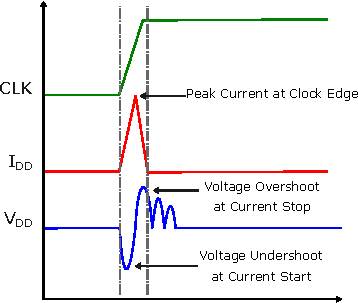
\includegraphics[scale=1.35, interpolate=false]
    {figures/villach-supply-analysis/chip-internal-oscillation}
    \caption[Chip-Internal Oscillation]{
        Chip-internal supply voltage oscillation at clock edges in a
        \ac{CMOS} circuit.
    }
    \label{fig:chip-internal-oscillation}
\end{figure}

In addition to the external power supply, the following factors contribute
to chip-internal voltage oscillations:

\begin{itemize}[topsep=8pt,itemsep=4pt,partopsep=4pt, parsep=4pt]
    \item
    The connection between external decoupling capacitors and on-chip
    switching nodes forms an effective RLC network, consisting of socket
    inductance, bond wire inductance and resistance, and chip-internal
    supply-to-ground capacitance \autocite{8919754}.

    \item
    Bond wire inductances limit the dynamic current delivery to the chip
    and convert fast load current transients into voltage drops and
    overshoots.

    \item
    Fast current transients generated at clock edges or during
    simultaneous switching events excite the RLC network, potentially
    leading to oscillatory behavior on internal supply rails.

    \item
    The slew rate of the load current determines the magnitude of the
    resulting voltage droop and subsequent voltage spike.

    \item
    Power-on and power-off transitions of internal power domains introduce
    additional current steps, which propagate through the chip-internal
    \ac{PDN} and package parasitics.

    \item
    Voltage droops become critical if the supply undershoot crosses
    digital noise margins for a duration sufficient to cause setup or
    hold time violations.
\end{itemize}

Low-impedance sockets, minimized bond wire inductance, and a well-designed
chip-internal \ac{PDN} help reduce internal voltage bounce. The speed and
stability of the \ac{DPS} control loop must be adapted to the overall
wiring length and parasitic elements of the test setup. Proper power
supply control loop design is therefore essential for reliable testing
and to minimize power-related anomalies.
%%%%%%%%%%%%%%%%%%%%%%%%%%%%%%%%%%%%%%%%%%%%%%%%%%%%%%%%%%%%%%%%%%%%%%%%%%%%%%%%%
%%%%%%%%%%%%%%%%%%%%%%%%%%%%%%%%%%%%%%%%%%%%%%%%%%%%%%%%%%%%%%%%%%%%%%%%%%%%%%%%%
%! Author = Saeid Yazdani
%! Date = 6/22/2024

%%%%%%%%%%%%%%%%%%%%%%%%%%%%%%%%%%%%%%%%%%%%%%%%%%%%%%%%%%%%%%%%%%%%%%%%%%%%%%%%


\section{Effects of Capacitive Loads}
\label{sec:capacitive-load-effects}

\ac{DUT} requires bypass capacitors to guarantee normal operation at
high power demand times as no control loop can ever counteract the nano-second
current demand of fast \ac{CMOS} circuitry.
Therefore, such current must be supplied from nearby power tanks – i.e.
capacitors.

When applying power to a \ac{DUT}, the \ac{DPS} supplies the \acs{DC}
current not only to the \ac{DUT}, but also the
decoupling capacitors and other elements of the circuit that
exhibit capacitive behaviour such as:

\begin{itemize}[topsep=8pt,itemsep=4pt,partopsep=4pt, parsep=4pt]
    \item Power plane capacitance
    \item Stray (parasitic) capacitances
    \item Other passive and active components sharing the power rail
\end{itemize}

A capacitive load affects the power supply control loop through
\emph{Charging Time} and \emph{Current Surge}.

\begin{itemize}[topsep=8pt,itemsep=4pt,partopsep=4pt, parsep=4pt]
    \item Charging time
    \item Current surge
\end{itemize}

Capacitors require a defined amount of time to charge up to a given voltage
($V_{max}$) which is dependent on the capacitance and resistance in
the circuit, known as \emph{Time Constant} or
\emph{RC Constant} ($\tau = {R \times C}$).
According to \autoref{eq:capacitor-charge-time}, a larger capacitance will have
a slower charging process which inherently increases settling time:

\begin{equation}
    \label{eq:capacitor-charge-time}
    V(t) = V_{\text{max}} \left(1 - e^{-\frac{t}{\tau}}\right)
\end{equation}

As a capacitor begins to charge the voltage across it increases
over time and asymptotically approaches $V_{max}$.
One multiple of RC Constant ($1\tau$) represents the time at which a capacitor
reaches approximately 63.2\% of $V_{max}$.
A capacitor is considered fully charged after $5\tau$ equal to 99.3\% of
$V_{max}$.
Reaching 100\% of the set voltage is limited by the internal losses denoted by
the exponential function, as shown in \autoref{fig:capacitor-charge-rc-curve}.

\begin{figure}[h]
    \centering
    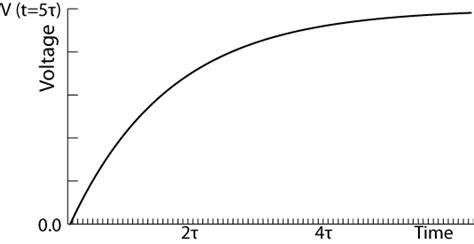
\includegraphics[scale=0.42]
    {figures/diagonostics/capacitor-charge-rc-curve}
    \caption[Capacitor Charging Curve]{
        The relationship between capacitor charging time and reaching a set
        voltage is asymptotic.
    }
    \label{fig:capacitor-charge-rc-curve}
\end{figure}


The time it takes for the capacitor to charge affects the feedback signal of
the power supply.
The control loop may not be able to react to the initial changes timely,
leading to an under-damped response and longer settling times.

When a capacitor begins to charge, it initially acts like a short circuit,
drawing a large surge current which affects the stability and response time of
power supply's control loop.
The momentary surge current is governed by the capacitance value as stated in
\autoref{eq:capacitor-current-surge}.

\begin{equation}
    \label{eq:capacitor-current-surge}
    I(t) = \frac{V_{\text{max}}}{R} e^{-\frac{t}{RC}}
\end{equation}

It should be noted that at $t=0$, the initial current is not influenced by the
capacitance value since $e^{-\frac{t}{RC}}=1$.
Rather it will be dependent on the applied voltage,
series resistance in the circuit wiring and \ac{ESR} of capacitors
as given in \autoref{eq:capacitor-current-surge-t0}.

\begin{equation}
    \label{eq:capacitor-current-surge-t0}
    I(0) = \frac{V_{\text{max}}}{R}
\end{equation}

The initial high current can momentarily overload the power supply
and can potentially engage the current limiting circuit of the power
supply, leading to disrupted output.
Furthermore, the inrush current can cause a voltage drop in the supply lines
due to their finite resistance, leading to an initial voltage sag that the
control loop must correct for.

The large initial current surge and subsequent rapid changes in current and
voltage can introduce phase shifts in the feedback loop, reducing the phase
margin and potentially causing instability or oscillations.

Inrush currents can cause instability and oscillation at power supply output
due to rapid changes in current and voltage which introduces \emph{Phase Shift}
in the control feedback loop, leading to a reduced phase margin.
Therefore, the prolonged settling time and the ringing observed in
\autoref{sec:dps-measurements} can mainly be attributed to charging time
and current surge due to the capacitance exhibited in the test setup.



%%%%%%%%%%%%%%%%%%%%%%%%%%%%%%%%%%%%%%%%%%%%%%%%%%%%%%%%%%%%%%%%%%%%%%%%%%%%%%%%%
%%%%%%%%%%%%%%%%%%%%%%%%%%%%%%%%%%%%%%%%%%%%%%%%%%%%%%%%%%%%%%%%%%%%%%%%%%%%%%%%%
%! Author = Saeid Yazdani
%! Date = 7/7/2024

\section{Effects of Current Limiting Circuits}
\label{sec:current-limiting-effects}

As stated before, in a typical \ac{ATE} setup, power supplies provide current to
both the DUT and its decoupling capacitors as well as parasitic capacitances.
The current going to the capacitors can significantly be based on the total
capacitance and power-up time set by the test developer.
As an example, powering up a \SI{3.3}{\volt} \ac{DUT} in \SI{100}{\micro\second}
with a total circuit capacitance of \SI{20}{\micro\farad} can need up to
\SI{1}{\ampere} according to \autoref{eq:current-during-capacitor-charge}.

\begin{equation}
    \label{eq:current-during-capacitor-charge}
    I = C \frac{dV}{dt}
\end{equation}

Almost all modern \ac{DPS} provide a programmable current limit option,
typically in \SI{10}{\milli\ampere} to \SI{50}{\milli\ampere} steps.
During test development and execution, it is a common practice to protect
\acp{DUT} from uncontrolled events by setting limits for the maximum current
a \ac{DPS} is allowed to source into a \ac{DUT}.

If a brief surge in current triggers a preset limit, the circuit will turn off
the limit once the surge stops, and the DPS will go back to providing the set
voltage with a delay.
Depending on the voltage level before the occurrence of a current surge event,
the actual voltage might need to go higher than the set voltage to make sure the
problem that caused the high current is settled.
Therefore the DUT might experience a voltage higher than the set
voltage for a short period.

If the test developer sets tight current limits, especially during the
\emph{TEST START} where all the capacitors need to be charged, there is a high
chance for misbehavior of the voltage rails due to the engagement of the current
limit circuitry.
This explains the presence of glitches
on \autoref{fig:villach-supply-analysis-1v3-test-start-glitch} and other
similar measurements.

\subsection{Mitigating Current-Limit Induced Glitching}
\label{subsec:current-limiting-effects}

As stated before, current depends on capacitance and how fast the voltage
changes, so the highest risk of engaging the current limit and overshooting
happens during power-up.
Test developers need to check power-up steps and the current limit.
Changing voltages by small amounts are less likely to be affected by the
capacitance and current limit because the voltage change is smaller.

The following points may help with reducing the overshoot and undershoot
triggered by the current limiting feature of a \ac{DPS}:

\begin{itemize}[topsep=8pt,itemsep=4pt,partopsep=4pt, parsep=4pt]
    \item \textbf{Relaxing the current limit:}
    Depending on internal circuitry and control loop of \ac{DPS} modules, test
    developers might need to increase current limits by at
    least \SI{100}{\milli\ampere} per microfarad to reduce the chance of
    high voltage glitches due to immature activation of current limit circuits.

    \item \textbf{Stepwise increase to target voltage:}
    Many modern \ac{DPS} allow for voltage step-ups with fine control over time
    taken by each step.
    If the \ac{DUT} power requirements allow, test developers can program the
    \ac{DPS} to reach target voltage in multiple steps, instead of one.

\end{itemize}













%%%%%%%%%%%%%%%%%%%%%%%%%%%%%%%%%%%%%%%%%%%%%%%%%%%%%%%%%%%%%%%%%%%%%%%%%%%%%%%%%
%%%%%%%%%%%%%%%%%%%%%%%%%%%%%%%%%%%%%%%%%%%%%%%%%%%%%%%%%%%%%%%%%%%%%%%%%%%%%%%%%
%! Author = Saeid Yazdani
%! Date = 7/26/2024


\section{Ganged-Mode Operation}
\label{sec:ganged-mode-operation}

The \ac{ATE} under investigation contains multiple \ac{DPS} units, each rated
at \SI{500}{\milli\ampere} maximum \acs{DC} current.
To supply larger currents to a \ac{DUT} with higher current demand,
multiple \ac{DPS} units must be connected in parallel
(so-called ganged mode) to increase the current output of the \ac{ATE}.

Ganged mode in power supplies is a configuration where multiple power supply
units are connected and operated together to form a cohesive system.
This mode of operation is designed to increase the total available
current in the form of load-sharing.
However, implementing gang mode comes with major challenges:

\begin{itemize}[topsep=8pt,itemsep=4pt,partopsep=4pt, parsep=4pt]
    \item \textbf{Complexity:}
    Design and implementation of a ganged configuration are more complex
    and requires much more wiring and components compared to a single power
    supply with higher output power.
    Precise calibration and voltage regulation also increases the design
    complexity.
    In addition, the overall software and firmware of the \ac{ATE} must
    be more sophisticated and therefore more error-prone.

    \item \textbf{Synchronization:}
    A perfect load balancing between multiple \ac{DPS} units in parallel is hard
    to achieve and can result in under-utilization or over-utilization of units.

    \item \textbf{Stability:}
    Small differences in output voltage between power supplies can result in
    circulating currents, leading to oscillations and instability
    due to subtle differences in impedance and phase angles caused by
    manufacturing tolerances which can not guarantee each participating
    \ac{DPS} in a ganged configuration to be exactly the same as others.
    Differences in transient response can also be expected if the participating
    units are not electrically matching.

    \item \textbf{\acs{EMI} Susceptibility:}
    Additional wiring and multiple power supplies can introduce noise and
    electromagnetic interference, which may affect the accuracy and
    performance of the ATE system and potentially couple into the \ac{DUT}.

    \item \textbf{Thermal management:}
    Multiple power supplies generate more heat, necessitating a robust
    cooling solution for the \ac{ATE}.
    Inadequate thermal management can lead to overheating and hinders the
    reliability and performance of the \ac{ATE}.

    \item \textbf{Cost:}
    More component count means higher production cost and higher maintenance
    cost are to be expected as identifying and troubleshooting issues can be
    more complex and time-consuming compared to a single power supply system.

\end{itemize}

\autoref{fig:ganged-mode-dps-structure} shows the block diagram of the DPS gang
configuration in the target \ac{ATE}.
In this mode, a DPS uses a master channel and one or more slave channels in
parallel to increase current output.
The master channel controls the output stages of the slave channels by
switching out their control amplifiers and connecting its own control amplifier
to them.

\begin{figure}[h]
    \centering
    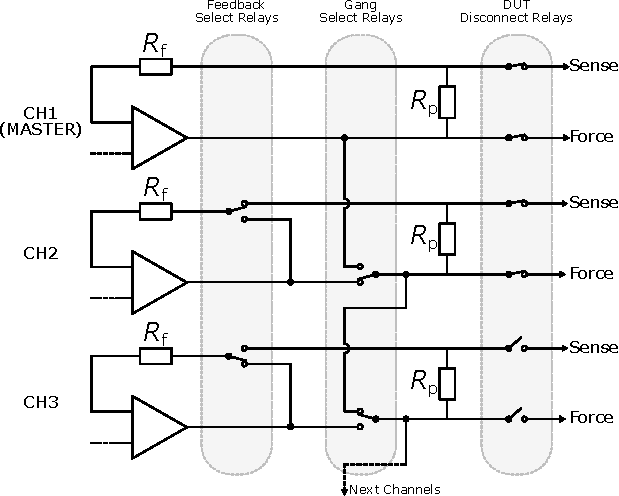
\includegraphics[width=0.9\textwidth]
    {figures/diagonostics/ganged_dps}
    \caption[Ganged DPS Structure]{
        Simplified block diagram of multiple \acs{DPS} channels with
        feedback and gang-select relays to form parallel structures.
        In this example, the first and second channels are engaged in
        ganged mode while the third channel is idle.
        $R_p$ Is a resistor in \SI{}{\mega\ohm} range to loosely couple sense
        feedback input to the force output when the sense terminal is disconnected,
        to prevent sudden output changes that can potentially damage the
        \ac{DUT}.
    }
    \label{fig:ganged-mode-dps-structure}
\end{figure}


Performing isolated measurements and comparing single channel to ganged-mode
operation yielded the following observations:

\begin{itemize}[topsep=8pt,itemsep=4pt,partopsep=4pt, parsep=4pt]
    \item
    Relays direct the master channel's control amplifier to each slave channel,
    closing all force and sense connections.

    \item
    Slave channels are in a temporary open-loop condition until the master
    amplifier is connected, and the slave force output links to the master
    sense input.

    \item
    The transition and settling of relays typically take up to
    \SI{5}{\milli\second}.

    \item
    During the open-loop state, the slave output goes from \SI{0}{\volt}
    to around \SI{1.5}{\volt}, increasing with the duration of the open-loop
    state.

    \item
    When the force relays of the slave channels close first, approximately
    \SI{1.5}{\volt} appears at the \ac{DUT} site.
    After the master channel's force and sense relays settle, the master adjusts
    the slave output voltage back to \SI{0}{\volt}.

\end{itemize}

These observations explain the glitches and the sudden rise to \SI{1.5}{\volt}
followed by a decay to \SI{0}{\volt} as seen in
\autoref{fig:villach-supply-analysis-1v3-test-start-with-dut}
and
\autoref{fig:villach-supply-analysis-5v0-test-start-with-dut}.















%%%%%%%%%%%%%%%%%%%%%%%%%%%%%%%%%%%%%%%%%%%%%%%%%%%%%%%%%%%%%%%%%%%%%%%%%%%%%%%%%
%! Author = Saeid Yazdani
%! Date = 6/22/2024


\section{\acs{DPS} Control Loop}
\label{sub:dps-control-loop}

All \ac{ATE} power supplies are programmable, and the output driver is inside a
control loop that will sense the target voltage at the \ac{DUT} site.
\emph{Remote Sense} is mandatory in the era of high supply currents and
low supply voltages – without remote sensing capabilities, there would be a
large unregulated voltage drop across the load board that would make the test
meaningless.

Systems such as \acp{ATE} which exhibit
significant wiring-related parasitics and variable \ac{DUT} load conditions must
use remote sensing schemes to compensate for voltage drops in the
cables between the power supply and the load, ensuring the correct voltage is
delivered at the load.

A comparison of control loops with and without remote sensing and the
associated errors is presented in
\autoref{fig:distributed-arrangement-ate-supply}:

\begin{itemize}[topsep=8pt,itemsep=4pt,partopsep=4pt, parsep=4pt]
    \item \textbf{Local Sense:}
    Without \emph{Remote Sense} and only relying on \emph{Local Sense}, we
    stabilize the supply voltage at the output of the source, and all wiring
    effects between source and \ac{DUT} are neglected.
    Such an arrangement is not suitable for precision measurements
    (\autoref{fig:distributed-arrangement-ate-supply}-A).

    \item \textbf{Basic Remote Sense:}
    If we can neglect all inductances of the sense lines because of very low
    settling times, we may succeed with a simple resistive approach
    (\autoref{fig:distributed-arrangement-ate-supply}-B).

    \item \textbf{Complex Remote Sense:}
    Because test times should be short, we need fast settling, and inductive
    components of the load board, socket and  \ac{DUT} can no longer be
    neglected (\autoref{fig:distributed-arrangement-ate-supply}-C).

\end{itemize}

\begin{figure}[htbp]
    \centering
    \printfitgraphics[0.62\textheight]{figures/villach-supply-analysis/distributed_arangement_ate_dut_supply}
    \caption[Comparison of Sensing Arrangements in Supplies]{
        The distributed arrangement of ATE source and DUT supply pin.
    }
    \label{fig:distributed-arrangement-ate-supply}
\end{figure}

While power supplies with remote sensing compensate for the wiring parasitic,
there are multiple challenges associated with such structures.
Implementing remote sensing requires additional wiring and components,
which will add complexity to the system design and in \ac{ATE} environments, and
requires dedicated wires on the load board to bring sense lines near the
\ac{DUT} socket.

This additional wiring introduces additional
susceptibility to noise and interference as incorrect or poor implementation of
remote sensing on any section of the \ac{ATE} to \ac{DUT} path can lead to
instability in the control loop and can potentially contribute to oscillations
and sporadic glitches seen in \autoref{ch:casestudy-from-ate-to-dut}.

Reducing analog components count and overall complexity of control loop in
favour of digital solutions can lead to a faster and more accurate transient
response.





%%%%%%%%%%%%%%%%%%%%%%%%%%%%%%%%%%%%%%%%%%%%%%%%%%%%%%%%%%%%%%%%%%%%%%%%%%%%%%%%%

\section{Conclusion}
\label{sec:diagnostics-conclusion}

In this chapter, we examined the factors causing problems with \ac{ATE}'s
\ac{DPS} units.
Some of the issues are caused by the load board design, but most are due to the
\ac{DPS} units struggling with capacitive loads and higher current demands.

Major glitches and unwanted voltages at the DUT site point to issues with
synchronizing multiple DPS channels, which is necessary for providing the
required current.

The analog control loop of the DPS is a major limitation.
Unlike digital systems, analog loops cannot be easily adjusted for each
\ac{DUT}'s characteristics to improve response times and compensate for load
conditions.
Analog loops are more prone to noise and drift, affecting performance and
stability.
They lack the precision and flexibility of digital systems, which can offer
more consistent operation and better performance through software adjustments.

Switching to digital control loops in DPS units could solve many of the
discussed problems.
Digital control offers advanced tools for real-time monitoring and
troubleshooting, making it easier to maintain and improve performance and are
more scalable and adaptable, better suited to handle the varying demands
of \ac{ATE} systems.

Furthermore, it is crucial to develop a solution with a sufficient current
output rating, eliminating the need for ganging configurations.
Avoiding ganging will reduce the synchronization and timing issues
related to relay switching and improve the overall reliability and simplicity
of the system.

In conclusion, to improve the reliability and performance of \ac{ATE} power
supplies, it is important to consider moving from analog to digital control
loops.
Additionally, we need to ensure that power supplies have enough current
output to avoid the complications of ganging.
This change would allow for more precise, adaptable, and stable power delivery,
improving the accuracy of test signals at the \ac{DUT} site.

In the following chapters, we will explore the concept of designing a hybrid
analog-digital \ac{DPS}, focusing on a time-variant control loop.
The discussion will include an evaluation of this approach and a detailed
insight into the implementation of a prototype.
This proposed solution aims to combine the strengths of both analog and
digital systems, potentially offering enhanced performance and
flexibility in \ac{ATE} power supplies.
